\chapter{Theoretical background} \label{chap:teoria}

In this chapter we present the theoretical background required to perform and interpret the simulations that follow. Before discussing Monte Carlo methods and specific update algorithms, we specify the system under study and the quantities used to characterise it. Starting from the physical origin of ferromagnetism and the ferromagnetic–paramagnetic phase transition, we introduce the Ising model and its Hamiltonian, define the relevant observables, and review the concepts (critical exponents, finite-size scaling, autocorrelation times) that underpin the analysis of the numerical results.

A ferromagnetic system is characterised by the alignment of microscopic magnetic moments (spins) in the same direction, producing a non-zero macroscopic magnetisation. Thermal fluctuations compete with this ordering: at low temperature spins tend to align, while at high temperature thermal disorder destroys the order. This competition gives rise to a critical temperature separating the ordered (ferromagnetic) and disordered (paramagnetic) phases. In the thermodynamic limit the transition is sharp, but in finite systems the singular behaviour is rounded and only approaches the ideal discontinuity as the system size increases.

We model the system in contact with a thermal reservoir at temperature $T$ and describe it using the canonical ensemble. Below we derive the expressions used to compute the physical observables from simulation data, formally define the Ising Hamiltonian, state the approximations and boundary conditions, and introduce the algorithms employed in this work.

\section{Ising model}

We now give a complete definition of the Ising model used throughout this work. The system is a two-dimensional square lattice with a classical spin $s_i\in\{+1,-1\}$ placed on each lattice site.
\begin{figure}
    \centering
    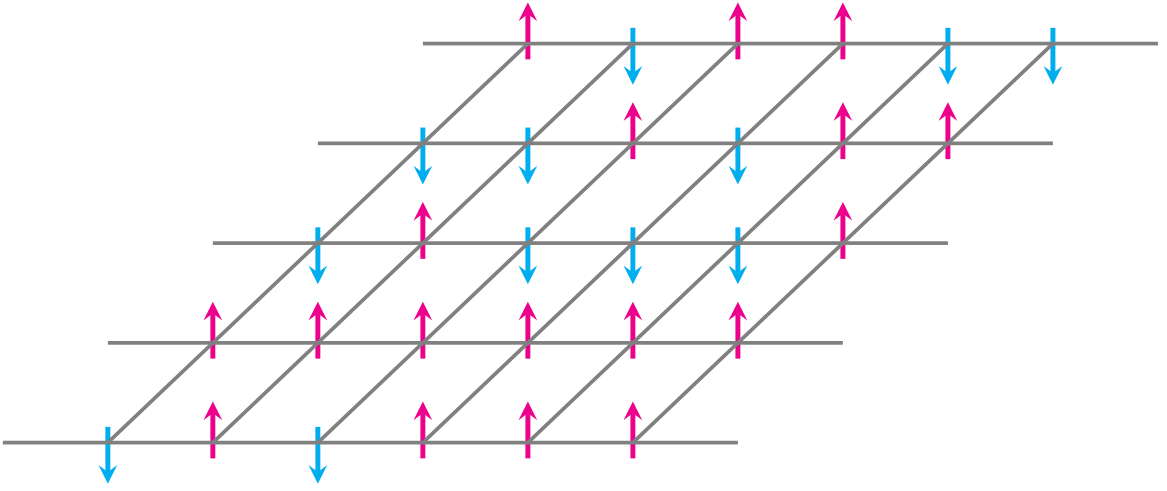
\includegraphics[width=0.7\textwidth]{fotos/2D_ising_model_on_lattice.svg.png}
    \caption{Example of a patch of the two-dimensional Ising lattice. \href{https://es.wikipedia.org/wiki/Modelo_de_Ising}{Source.}}
    \label{fig:ising-red}
\end{figure}
The general Hamiltonian reads
\[
\mathcal{H} = -J\sum_{\langle i,j \rangle} s_i s_j - H\sum_i s_i,
\]
where $s_i=\pm1$ is the spin at site $i$, $J$ is the coupling constant and $H$ is a uniform external magnetic field. The first sum runs over nearest-neighbour pairs and the second over all sites.

For $J>0$ the ground state is ferromagnetically ordered, while $J<0$ favours antiferromagnetic order. In this work we study the ferromagnetic case without external field ($H=0$), so the Hamiltonian simplifies to $\mathcal{H}=-J\sum_{\langle i,j\rangle}s_i s_j$ with nearest-neighbour interactions only.

The natural order parameter for the transition is the magnetisation per spin,
\[ m=\frac{1}{N}\sum_i s_i, \]
with $N=L^2$ the total number of spins. In the thermodynamic limit $m=0$ for $T>T_c$ and $m\neq0$ for $T<T_c$. In finite systems global spin-inversion symmetry implies $\langle m\rangle=0$ for all $T$, so in simulations one typically uses $\langle|m|\rangle$ as the estimator of the order parameter.

\section{Mecánica estadística}

In the canonical ensemble the equilibrium state of a system in contact with a heat bath at temperature $T$ is specified by the partition function
\[
Z=\sum_{\{\sigma\}} e^{-\beta\mathcal{H}(\sigma)},
\]
with $\beta=1/(k_B T)$ and the sum over all microstates $\{\sigma\}$. Thermodynamic quantities follow from $Z$; for instance the free energy $F=-k_B T\ln Z$, and the average energy
\[ \langle E \rangle = -\frac{\partial \ln Z}{\partial \beta}. \]
The heat capacity per spin can be written in terms of energy fluctuations as
\begin{equation} \label{eq:Cv}
    c = \frac{1}{N}\frac{\partial \langle E \rangle}{\partial T} = \frac{1}{N k_B T^2}\left(\langle E^2 \rangle - \langle E \rangle^2\right).
\end{equation}
Similarly, the magnetic susceptibility per spin is related to magnetisation fluctuations,
\[ \chi = \frac{1}{N k_B T}\left(\langle M^2 \rangle - \langle M \rangle^2\right), \]
with $M=\sum_i s_i$ the total magnetisation. These relations are used to compute $c$ and $\chi$ from time-series produced by the simulations.

We also use the fourth-order Binder cumulant,
\[ U_4 = 1 - \frac{\langle m^4 \rangle}{3\langle m^2 \rangle^2}, \]
which is dimensionless and takes a universal value at $T_c$ depending only on the universality class and boundary conditions; this makes it a convenient tool to locate the critical temperature in finite systems (see Sec.~\ref{sec:fss}).

The correlation length $\xi_L$ measures the typical distance over which spin fluctuations are correlated and can be obtained from the spin–spin correlation function $g(r)=\langle s_0 s_r\rangle-\langle s_0\rangle\langle s_r\rangle$, which decays approximately exponentially away from $T_c$, $g(r)\sim e^{-r/\xi_L}$. In finite periodic lattices it is practical to use the second-moment correlation length \citep{Cooper1982, Newman1999}, built from the structure factor
\begin{equation} \label{eq:structure_factor}
    \chi(\mathbf{k}) = \frac{1}{N}\left\langle \left| \sum_j s_j\, e^{i\mathbf{k}\cdot\mathbf{r}_j} \right|^2 \right\rangle,
\end{equation}
evaluated at $\mathbf{k}=0$ and at the smallest non-zero wavevector $k_{\min}=2\pi/L$. The second-moment correlation length is then
\begin{equation} \label{eq:xi_def}
    \xi_L = \frac{1}{2\sin(\pi/L)}\sqrt{\frac{\chi(0)}{\chi(k_{\min})} - 1}.
\end{equation}
This definition is convenient because it can be computed directly from configurations sampled during the simulation without evaluating $g(r)$ for every distance.

Expected values appearing in the above formulas are phase averages,
\[ \langle O \rangle = \frac{1}{Z}\sum_{\{\sigma\}} O(\sigma) e^{-\beta\mathcal{H}(\sigma)}, \]
which are not computed directly by summation over the $2^N$ microstates but estimated via importance sampling. A Markov-chain Monte Carlo algorithm generates a sequence of configurations $\sigma_1,\dots,\sigma_M$ distributed according to the Boltzmann weight once equilibrium is reached. Provided the chain is ergodic and satisfies detailed balance (conditions enforced by the algorithms described in Sec.~\ref{sec:montecarlo}), phase averages are obtained as time averages over the sampled configurations:
\[ \langle O \rangle \approx \frac{1}{M}\sum_{t=1}^M O(\sigma_t), \]
where $\sigma_t$ denotes the full spin configuration at the $t$-th measurement after thermalisation and $M$ is the number of measurements.


% =======================================================================================


\section{Phase transition, critical temperature and critical exponents}

In the thermodynamic limit the 2D Ising model undergoes a phase transition exactly at $T_c$ (eq.~\ref{eq:Tc_onsager}). Near this point thermodynamic quantities become non-analytic. In particular, the correlation length diverges as
\[ \xi(T)\sim|T-T_c|^{-\nu}, \]
and other observables follow power laws with their characteristic exponents: the magnetisation behaves as $m\sim(T_c-T)^{\beta}$ for $T<T_c$, the susceptibility as $\chi\sim|T-T_c|^{-\gamma}$, and the heat capacity as $c\sim|T-T_c|^{-\alpha}$. For the 2D Ising model the heat-capacity divergence is only logarithmic, corresponding to $\alpha=0$.

The exponents $\nu,\beta,\gamma,\alpha$ are called critical exponents and arise because at $T_c$ the correlation length diverges and the system has no intrinsic length scale. Consequently the critical behaviour depends only on dimensionality and symmetry of the order parameter, not on microscopic details — the phenomenon of universality \citep{Wilson1974}. The 2D Ising model belongs to a well-known universality class with exact exponent values (Onsager and subsequent results \citep{Yang1952}):
\[ \nu=1,\quad \gamma=\frac{7}{4}. \]
These values serve as references for comparing the numerical estimates from simulations.

\section{Finite-size scaling} \label{sec:fss}

The divergences mentioned above occur only in the limit $L\to\infty$. In a finite system the correlation length cannot exceed the system size and saturates at $\mathcal{O}(L)$ near $T_c$, so thermodynamic quantities are smooth functions of $T$. Finite-size scaling (FSS) theory \citep{Fisher1972} assumes that when $\xi\sim L$ the only relevant ratio is $L/\xi$, and any observable can be expressed as a scaling form depending on $(T-T_c)L^{1/\nu}$. For our observables
\[ \langle|m|\rangle(L,T)=L^{-\beta/\nu} f_m\big((T-T_c)L^{1/\nu}\big), \]
\begin{equation} \label{eq:fss_chi2}
    \chi(L,T)=L^{\gamma/\nu} f_\chi\big((T-T_c)L^{1/\nu}\big),
\end{equation}
\begin{equation} \label{eq:fss_xi2}
    \xi_L(L,T)=L f_\xi\big((T-T_c)L^{1/\nu}\big),
\end{equation}
where $f_m,f_\chi,f_\xi$ are universal scaling functions. Plotting appropriately rescaled observables (e.g. $\chi L^{-\gamma/\nu}$) against $(T-T_c)L^{1/\nu}$ for different $L$ should collapse the curves onto a single universal function when the correct exponents and $T_c$ are used, providing a direct test of universality.

Finite-size effects also shift pseudocritical temperatures: peak positions for $\chi$ or $c$ occur at $T_c(L)$ satisfying
\[ T_c(L)-T_c\sim L^{-1/\nu}. \]
The Binder cumulant $U_4=1-\langle m^4\rangle/(3\langle m^2\rangle^2)$ \citep{Binder1981} is dimensionless and scales as $U_4(L,T)=f_U\big((T-T_c)L^{1/\nu}\big)$, so its curves for different $L$ should cross at $T_c$, enabling an estimate of the critical temperature without fitting other exponents.

\section{Autocorrelation time} \label{sec:csd}

We clarify the notion of "time" used here. Monte Carlo simulations do not reproduce real microscopic dynamics; configurations are generated by stochastic update rules. Therefore the "time" index is simply the sequence index measured in Monte Carlo steps (Sec.~\ref{sec:pasomc}). It is a discrete, dimensionless, algorithm-dependent unit. In what follows any temporal scale is measured in MCS.

The generated sequence $\sigma_1,\sigma_2,\dots,\sigma_M$ is temporally correlated since each configuration is obtained from the previous one by small updates. Correlations for an observable $O$ are quantified by the autocorrelation function \citep{LandauBinder}
\[ C_O(t)=\langle O(t_0)O(t_0+t)\rangle-\langle O\rangle^2, \]
which typically decays exponentially $C_O(t)\sim e^{-t/\tau_O}$, where $\tau_O$ is the autocorrelation time associated to $O$. Larger $\tau_O$ means more MCS must be skipped between measurements to obtain effectively independent samples: the effective number of independent measurements is approximately $M/(2\tau_O)$ rather than $M$.

Near $T_c$, where $\xi$ grows, autocorrelation times also increase (critical slowing down), described by the dynamic exponent $z$ \citep{HohenbergHalperin1977}:
\[ \tau\sim\xi^z\sim L^z. \]
Unlike static exponents, $z$ depends on both universality class and the update algorithm. Local algorithms such as Metropolis or Glauber have relatively large $z$ for the 2D Ising model ($z\approx2.17$), while cluster algorithms \citep{SwendsenWang1987} like Wolff reduce $z$ substantially. This difference in $\tau(L)$ near criticality is a central aspect of our algorithmic comparison.

In practice we compute the normalized autocorrelation function
\[ \rho_O(t)=\frac{C_O(t)}{C_O(0)}, \]
and the integrated autocorrelation time
\begin{equation} \label{eq:tau_int}
    \tau_{\mathrm{int},O}=\frac{1}{2}+\sum_{t=1}^{\infty}\rho_O(t),
\end{equation}
which determines the true variance of the sample mean:
\[ \mathrm{Var}(\langle O\rangle)\approx\frac{2\tau_{\mathrm{int},O}}{M}\mathrm{Var}(O). \]
The sum in eq.~\eqref{eq:tau_int} must be truncated in practice at some cutoff $t^*$ where $\rho_O(t)$ has sufficiently decayed; choosing $t^*$ requires care to avoid under- or overestimating $\tau_{\mathrm{int},O}$ due to noise.